\section{Results}
\label{section:results}

In Fig. \ref{fig:sdip} we present the computed
single and double ionization spectra
of strontium in order to analyze the possible decay channels. The main peaks of the
ionization
from the Sr$4p_{3/2}$ and the Sr$4p_{1/2}$ have single ionization potentials (SIP)
of \unit[28.277]{eV} and \unit[29.402]{eV}, respectively. These energies are higher
than only one double ionization potential (DIP) of \unit[16.430]{eV},
which is to \unit[99.7]{\%} characterized by the double ionization from
the $5s$ valence. The Auger process is therefore energetically accessible.
For radium the spectra are qualitatively the same and
allow the same conclusion. The single ionization energies and polestrengths
of the main
peaks of the intial ionizations are collected in Table \ref{tab:widths}.

\begin{figure}[h]
 \centering
 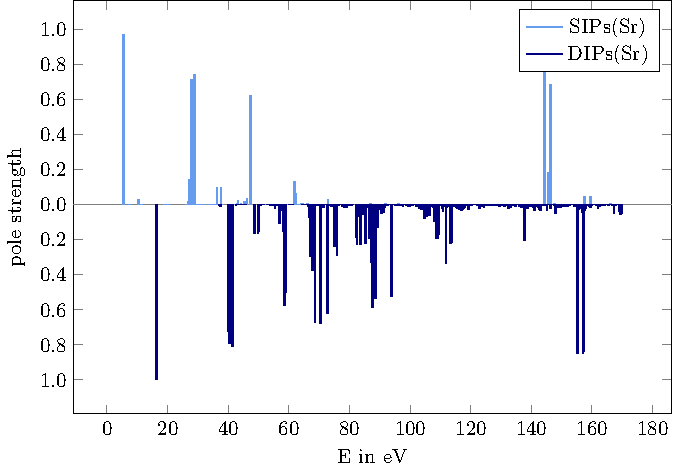
\includegraphics[width=\columnwidth]{pics/Sr_rel_sdip.pdf}
 \caption{Comparison of the single (SIP) and double (DIP) ionization spectra
          of the strontium obtained by a DC-ADC calculation.}
 \label{fig:sdip}
\end{figure}

\begin{table}[h]
 \centering
 \caption{}
 \begin{tabular}{lrrr}
  \toprule
   initial state    & energy $[\unit{eV}]$ & ps & $\Gamma [\unit{meV}]$\\
  \midrule
   Sr spinfree      & 28.599 & 0.78 &   0.56\\  
   Sr$4p_{1/2,1/2}$ & 29.402 & 0.80 &   0.10\\
   Sr$4p_{3/2,1/2}$ & 28.277 & 0.76 &   1.23\\
   Sr$4p_{3/2,3/2}$ & 28.277 & 0.76 &   1.17\\
%  \midrule
%   Ba$5p_{1/2,1/2}$ & 25.108 & 0.80 & unreliable\\
%   Ba$5p_{3/2,1/2}$ & 23.106 & 0.76 &   55.9\\
%   Ba$5p_{3/2,3/2}$ & 23.106 & 0.76 &   63.1\\
  \midrule
   Ra spinfree      & 21.836 & 0.49 &  28.56 \\  
   Ra$6p_{1/2,1/2}$ & 25.494 & 0.78 &   0.26\\
   Ra$6p_{3/2,1/2}$ & 19.267 & 0.50 &  93.16 \\
   Ra$6p_{3/2,3/2}$ & 19.267 & 0.50 &  98.86\\
  \bottomrule
 \end{tabular}
 \label{tab:widths}
\end{table}


We present the decay widths of strontium and radium in Table \ref{tab:widths}
for the scalarrelativistic spinfree $(n-1)p^{-1}$ as well as the
fully relativistic $(n-1)p_{1/2,1/2}^{-1}$, $(n-1)p_{3/2,1/2}^{-1}$ and
$(n-1)p_{3/2,3/2}^{-1}$ initial states. They are illustrated in Fig. \ref{fig:gamma}.
To the best of my knowledge, the Auger decay widths of these systems have
not been presented in the literature so far, even though xyz compare their
radiative lifetimes to Auger widths, which they seem to have gained
from private communication with xyz \cite{}.
Despite the difference in absolute numbers, the different decay widths
of the different initial states show the same pattern. The decay width of
the $(n-1)p_{1/2,1/2}^{-1}$ initial state is lowest, while the decay widths
of the $(n-1)p_{3/2,1/2}^{-1}$ and
$(n-1)p_{3/2,3/2}^{-1}$ initial states are close and significantly higher than
for the $(n-1)p_{1/2,1/2}^{-1}$ initial state. The decay widths of the
spinfree calculations is in between these values.
How can this result be understood?

\begin{figure}[h]
 \centering
 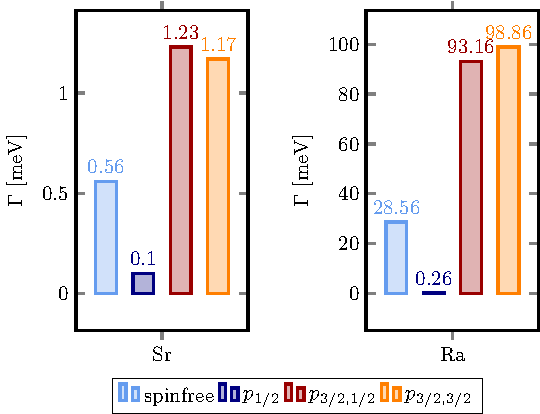
\includegraphics[width=0.95\columnwidth]{pics/gamma_group.pdf}
 \caption{}
 \label{fig:gamma}
\end{figure}

Considering our previous findings about the role
of scalarrelativistic effects on electronic decay widths \cite{Fasshauer15_1},
we inspect the radial densities of the $(n-1)p$ and the $ns$ orbitals of the
strontium and radium ions,
which we assume to be involved in the decay process (see
Fig.~\ref{fig:radial_pure}).
In case of the strontium atom, the radial densities of the $4p_{1/2}$ and the
$4p_{3/2}$ orbitals are almost identical. But for the radium atom, the radial
density of the  $6p_{1/2}$ orbital is located closer to the nucleus than
the radial density of the $6p_{3/2}$ orbital. This general property is already
visible in the analytic solutions of the one-electron system \cite{Bethe_Salpeter}.
Because the Auger decay rates depend crucially depend on the overlap of the
involved orbitals, the decay widths of an $(n-1)p_{3/2}^{-1}$ initial state
can be expected to be higher than the decay widths of an $(n-1)p_{1/2}^{-1}$
initial state. These findings are reflected in the decay widths shown in
Fig.~\ref{fig:gamma} and Table \ref{tab:widths} and is consistent with the
observations of the noble gas Auger processes in Ref. \cite{Fasshauer15_1}.


\begin{figure}[h]
 \centering
 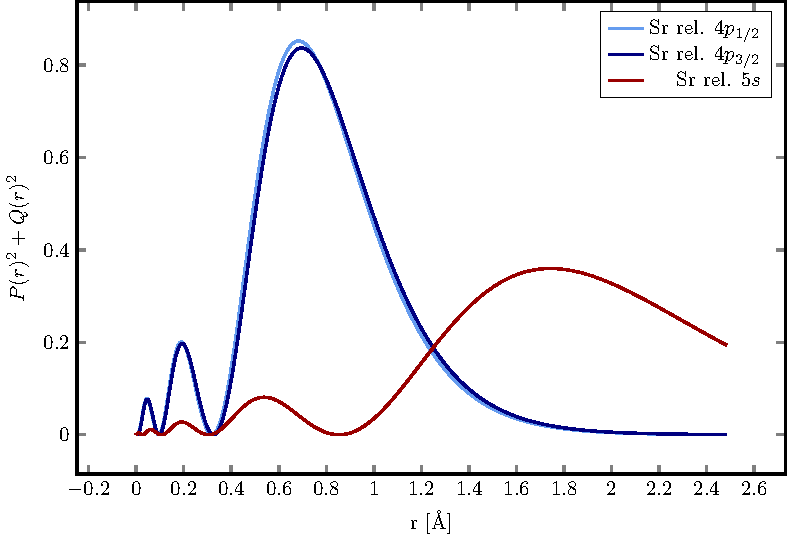
\includegraphics[width=\columnwidth]{pics/sr_ion_R.pdf}\\
 %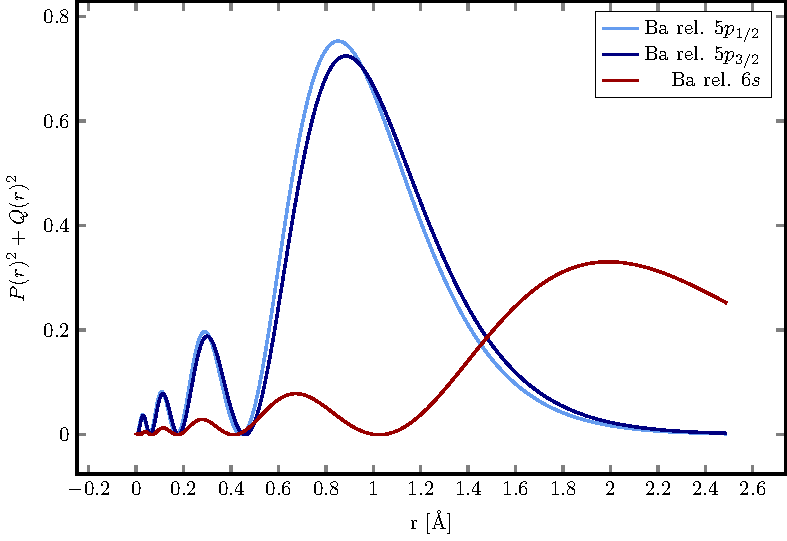
\includegraphics[width=\columnwidth]{pics/ba_ion_R.pdf}\\
 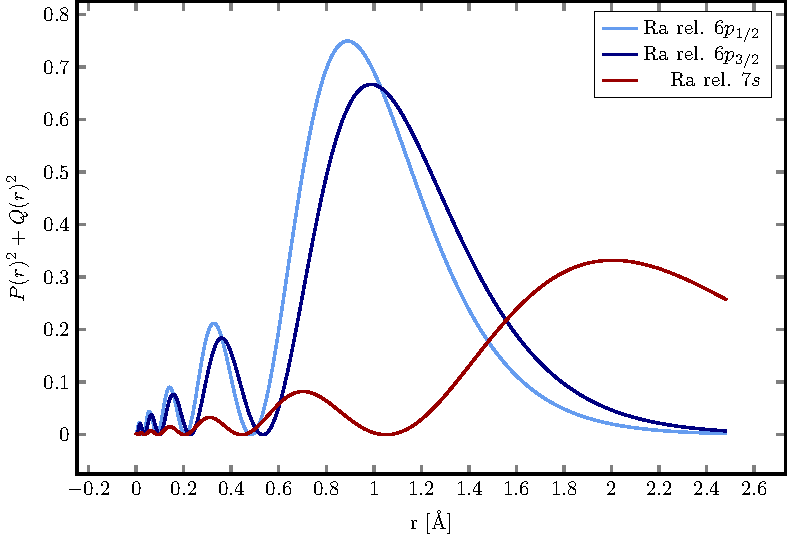
\includegraphics[width=\columnwidth]{pics/ra_ion_R.pdf}\\
 \caption{Radial densities of the orbitals of the $(n-1)p^5s^2$ ions
          involved in the Auger decay.
          The expectation value of the electrons position of the $(n-1)p_{1/2}$
          orbital is lower than of the respective $(n-1)p_{3/2}$
          orbitals. The $ns$ orbitals of the ions experience a stronger
          contraction the those of the atom (not shown here).}
 \label{fig:radial_pure}
\end{figure}

However, the simulations of Auger processes in other earthalkaline elements
have shown that configuration interactions are important for the correct
description of these elements' decay widths. Both the investigations of
the Auger process following primary ionization
from the $2p$ orbitals of calcium \cite{}
as well as the from the $4d$ orbitals of barium \cite{}
showed the necessity to include excitations from the valence $s$ orbital to
the $d$ orbitals, which are unpopulated in the ground state, in the
description of the initial state.
In our case, this would require to include the following processes in our
simulations:

\begin{align*}
 (n-1)p^{-1} \,ns^2         \rightarrow & (n-1)p^6 + e^- \\
 (n-1)p^{-1} \,(n-1)d \, ns \rightarrow & (n-1)p^6 + e^- \\
 (n-1)p^{-1} \,(n-1)d^2     \rightarrow & (n-1)p^6 + e^- .
\end{align*}

Indeed, the analysis of the ADC eigenvectors of the initial states of both
strontium and radium showed,
that beyond the single and main $1h$ contribution of the respective $p$ orbital, the
initial state is mainly characterized by $2h1p$ configurations of the
$(n-1)p^{-1} \,ns \, (n-1)d$ kind and the $(n-1)p^{-1} \,(n-1)d \, ns$
configurations are therefore automatically included in our simulations.
The FanoADC-Stieltjes approach is however limited
to perturbation theory of second order, which are further corrected by third order
terms, but does not go beyond $2h1p$ configurations. This means, that the
$(n-1)p^{-1} \,(n-1)d^2$ configurations are not taken into account in this work.

How do these configurations affect the decay widths? Since the overlap of the
orbitals involved in the decay determine the decay widths, we show the
radial densities of the orbitals involved in the decay of the $6p^5 6d 7s$
configuration of radium in Fig.~\ref{fig:radial_ra}.
The radial densities of the $6p$ and $7s$ orbitals hardly differ from the
corresponding radial densities of the ionic $6p^{-1} \,7s^2$ configurations
shown in Fig.~\ref{fig:radial_pure}. However, the $6d$ orbitals, which are involved
of the Auger process of this configuration shows a larger overlap with both
the $6p$ and the $7s$ orbitals. The corresponding decay width should therefore
be larger than the decay width of the $6p^{-1} \,7s^2$ configuration.
The prevalence of the $(n-1)p_{3/2}$ decay width over the $(n-1)p_{1/2}$
also holds for this configuration.
If the $(n-1)p^{-1} \,(n-1)d^2$ configurations would turn out to
have non-negligible contributions
in a more accurate calculation,
the presented decay widths of Table~\ref{tab:widths} would then be
lower bounds to the real decay widths.

\begin{figure}[h]
 \centering
 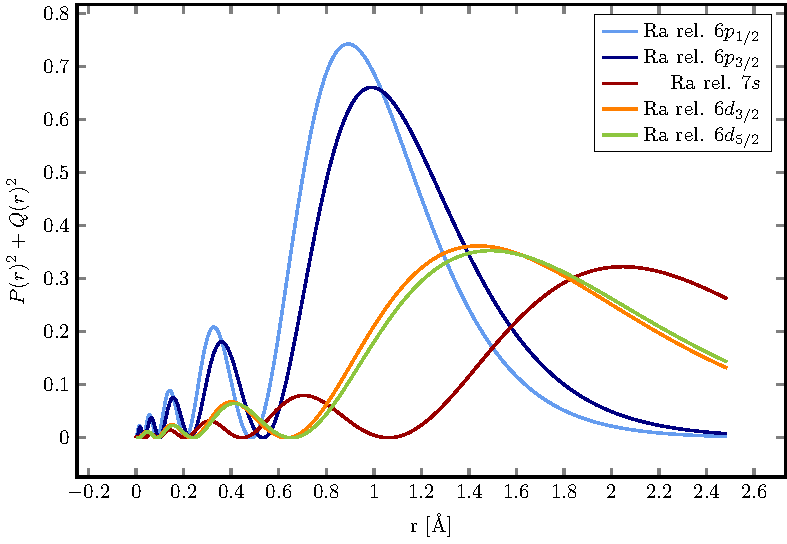
\includegraphics[width=\columnwidth]{pics/ra_6d_R.pdf}
 \caption{Radial densities of the radium orbitals of the ionic $6p^5 6d 7s$
          configuration involved in the Auger decay. The overlap of the radial
          densities of the $6p$ orbitals with the radial densities of the $6d$ orbitals
          is more pronounced than with the radial density of the $7s$ orbital.}
 \label{fig:radial_ra}
\end{figure}

The observed differences in the decay widths for different initial states and
Hamiltonians can therefore not necessarily only be accounted for by relativistic
effects, but different contributions of the $(n-1)p^{-1} \,(n-1)d \, ns$
configurations may also affect the result.
The pole-strength, i. e., the absolute square of the $1h$ coefficients,
of the different initial states are
given in Table \ref{tab:widths}.
Since the analysis of the eigenvectors has shown the other significant contributions
to be of the $(n-1)p^{-1} \,ns \, (n-1)d$ kind, we for our discussion assume, that
they are the only other contributions.
For strontium, the pole-strengths are similar, but not identical for all initial
states and Hamiltonians. For radium, however, the pole-strengths are very different.
The $6p_{1/2}$ initial state has a pole-strength of 0.78, while both the
initial state of the scalarrelativistic Hamiltonian and the $6p_{3/2}$ initial
state have much lower pole-strengths of 0.49 and 0.50, respectively.
The $6p^{-1} \,7s^2$ configuration is therefore predominant for the $6p_{1/2}$
initial state, while it is not for the $6p_{3/2}$ initial state. This could
explain the observed discrepancy of decay widths of the $6p_{3/2}$ and
$6p_{1/2}$ initial states. However, the initial state determined with the spinfree
Hamiltonian has a comparable pole-strength, but a significantly lower decay
width. We can therefore conclude that the spin-orbit coupling does affect
the Auger decay widths, even though it is not the only factor for the case of
earth alkaline atoms.


